\documentclass[11 pt]{book}
\usepackage[utf8]{inputenc}
\usepackage[spanish]{babel}
\usepackage{graphicx}
\usepackage[margin=2.5cm]{geometry}
\usepackage{color}
\usepackage{pdfpages}
\begin{document}
\title{\textbf {\Huge Memoria del proyecto Polis}}
\author{
	\textbf {Ingeniería del Software de Gestión II - Grupo 10 - Iteración 6}\\\\
	Samuel Navas Portillo\\
	Juan Jesús Pérez Luna\\
	Manuel de los Santos Campos\\
	María José Sancha Maya\\
	Ángel Martínez Olivares\\
	José Antonio Jiménez Carmona}
\maketitle
\tableofcontents{}

\chapter{Vídeo explicativo del juego}
	El siguiente vídeo online explica brevemente cómo se juega al juego de mesa Polis.\\ \\
	\texttt{http://www.youtube.com/watch?v=gTCdMBfJiHo}
	
\chapter{Planificación Temporal}
	En una primera conversación del grupo realizada el 29 de Septiembre, se llega al siguiente acuerdo sobre la planificación de las reuniones regulares del grupo y de las distintas entregas del proyecto:\\

    \section{Reuniones ordinarias}
        \subsection*{Iteración 1}
	        Cada martes de 9:30 a 11:30 y/o viernes de 12:30 a 14:30 de cada semana hasta que tenga lugar la última entrega del proyecto, el grupo debe reunirse para analizar el estado del proyecto y del grupo y, en su caso, discutir y tomar las decisiones que e tomen oportunas.\\

    \section{Entregas de las iteraciones}
        \subsection*{Iteración 1}
            La primera entrega del proyecto será el día 7 de Octubre de 2010. Las siguientes entregas serán, respectivamente, los días 20 de Octubre, 29 de Octubre, 5 de Noviembre, 12 de Noviembre, 19 de Noviembre, 26 de Noviembre, 3 de Diciembre, 10 de Diciembre, 17 de Diciembre y, por último, 14 de Enero.
            
        \subsection*{Iteración 2}
            La primera entrega del proyecto será el día 7 de Octubre de 2010. Las siguientes entregas (2ª y 3ª Iteración) serán, respectivamente, los días 14 de Octubre y 21 de Octubre respectivamente.
            
        \subsection*{Iteración 3}
	        La primera entrega del proyecto será el día 7 de Octubre de 2010. Las siguientes entregas (2ª y 3ª Iteración) serán, respectivamente, los días 14 de Octubre y 11 de noviembre respectivamente.

		\subsection*{Iteración 4}
			La entrega de la 4ª iteración será el día 3 de Diciembre.
			
		\subsection*{Iteración 5}
			La entrega de la 5ª iteración será el día 18 de Diciembre.
			
		\subsection*{Iteración 6}
			La entrega de la 6ª iteración será el día 11 de Enero.
			
	\section{Reuniones extraordinarias}
	    \subsection*{Iteración 1}
		    El martes 5 de Octubre (de 17:30 a 20:30) y el miércoles 6 de Octubre (de 9:00 a 11:30, de 15:30 a 17:30 y de 19:30 a 21:30) tuvimos 2 reuniones extra respectivamente.

\chapter{Memorando técnico}
	Este capítulo presenta un breve resumen de las actividades realizadas en cada iteración o etapa.
	
	\subsection*{Iteración 1}
		En esta primera etapa se ha estudiado las reglas del juego, construído el juego de mesa y producido un vídeo explicativo del juego.
		
	\subsection*{Iteración 2}
		Las actividades principales fueron el repaso del temario impartido por la asignatura Ingeniería del Software 1 y el diseño del diagrama UML de análisis del proyecto.
		
	\subsection*{Iteración 3}
		En este tiempo se diseñó el diagrama UML de diseño del proyecto, se modificó el diagrama UML de análisis del proyecto, se realizó el diagrama de asignación de responsabilidades y se preparó el entorno técnico (Eclipse y Subversion) para el desarrollo del proyecto.
		
	\subsection*{Iteración 4}
		En esta iteración se modificó el diagrama de asignación de responsabilidades y se implementó la arquitectura de código del proyecto y parte de sus clases y funciones.
	
	\subsection*{Iteración 5}
		En esta etapa se ha completado el código del proyecto hasta terminarlo. Para la próxima etapa, queda pendiente la refactorización de algunas partes del código
		
	\subsection*{Iteración 6}
		Esta fase nos ha llevado a refactorizar el código del proyecto en una gran parte (incluída la interfaz de usuario de consola), para hacer de éste un código más legible, más modular, con menos acoplamiento y más reutilizable. Esta iteración ha supuesto un esfuerzo bastante grande para el grupo ya que ha sido necesario un análisis de todo el proyecto en profundidad, ya que no era trivial determinar qué partes del código había que cambiar. También, en fase parte del desarrollo, hemos realizado las primeras pruebas de ejecución completa del programa, es decir, hemos usado el programa tomando el papel de usuarios para comprobar que funcionaba correctamente.
		
\chapter{Seguimiento}
	Este capítulo presenta las actividades concretas realizadas por cada miembro del grupo así como su tiempo invertido.
	
	\section{Actividades}
	    \subsection*{Iteración 1}
		    \begin{itemize}
			    \item \textbf {Samuel Navas Portillo}
				    \begin{enumerate}
					    \item Búsqueda de materiales: \textbf{1h 30min}
					    \item Fabricación de las fichas y cartas del juego: \textbf{2h}
					    \item Lectura de las Normas: \textbf{1h}
					    \item Impresión de las Normas del juego: \textbf{1h 30min}
					    \item Simulación de partidas: \textbf{2h}
					    \item Guión del vídeo (1ª parte): \textbf{2h}
					    \item Guión del vídeo (2ª parte): \textbf{2h}
				    \end{enumerate}
			    \item \textbf {Juan Jesús Pérez Luna}
				    \begin{enumerate}
					    \item Análisis y síntesis de las Normas del juego: \textbf{3h}
					    \item Impresión del juego: \textbf{30min}
					    \item Fabricación de las fichas y cartas del juego: \textbf{2h}
					    \item Lectura de las Normas: \textbf{1h}
					    \item Simulación de partidas: \textbf{2h}
					    \item Guión del vídeo y actor (mano) (1ª parte): \textbf{2h}
					    \item Guión del vídeo (2ª parte): \textbf{1h}
				    \end{enumerate}
			    \item \textbf {Manuel de los Santos Campos}
				    \begin{enumerate}
					    \item Lectura de las Normas: \textbf{2h}
					    \item Simulación de partidas: \textbf{2h}
					    \item Guión del vídeo (1ª parte): \textbf{2h}
					    \item Guión del vçideo y actor (mano) (2ª parte): \textbf{2h}
				    \end{enumerate}
			    \item \textbf {María José Sancha Maya}
				    \begin{enumerate}
					    \item Búsqueda y preparación del equipo de grabación del video: \textbf{30min}
					    \item Fabricación tablero: \textbf{2h}
					    \item Lectura de las Normas: \textbf{1h}
					    \item Simulación de partidas: \textbf{2h}
					    \item Guión del vídeo (1ª parte): \textbf{2h}
					    \item Grabación del vídeo (cámara): \textbf{2h}
					    \item Edición del vídeo (postproducción): \textbf{5h}
				    \end{enumerate}
			    \item \textbf {Ángel Martínez Olivares}
				    \begin{enumerate}
					    \item Búsqueda de materiales: \textbf{1h 30min}
					    \item Fabricación de las fichas y cartas del juego: \textbf{2h}
					    \item Lectura de las Normas: \textbf{1h}
					    \item Simulación de partidas: \textbf{2h}
					    \item Guión del vídeo y actor (voz) (1ª parte): \textbf{2h}
					    \item Guión del vídeo y actor (voz) (2ª parte): \textbf{3h}
				    \end{enumerate}
			    \item \textbf {José Antonio Jiménez Carmona}
				    \begin{enumerate}
					    \item Impresión del juego: \textbf{30min}
					    \item Fabricación de las fichas y cartas del juego: \textbf{2h}
					    \item Lectura de las Normas: \textbf{1h}
					    \item Simulación de partidas: \textbf{1h 30min}
					    \item Guión del video (1ª parte): \textbf{2h}
					    \item Aprendizaje básico de "Latex" y producción de la Memoria (versión 1.0): \textbf{4h}
				    \end{enumerate}
		    \end{itemize}
		    
		\subsection*{Iteración 2}
		    \begin{itemize}
			    \item \textbf {Samuel Navas Portillo}
				    \begin{enumerate}
					    \item Estudio/repaso del tema de análisis de Ingeniería del Software de Gestión 1 y propuesta de diseño UML: \textbf{10h}
				    \end{enumerate}
			    \item \textbf {Juan Jesús Pérez Luna}
				    \begin{enumerate}
					    \item Estudio/repaso del tema de análisis de Ingeniería del Software de Gestión 1 y propuesta de diseño UML: \textbf{10h}
				    \end{enumerate}
			    \item \textbf {Manuel de los Santos Campos}
				    \begin{enumerate}
					    \item Estudio/repaso del tema de análisis de Ingeniería del Software de Gestión 1 y propuesta de diseño UML: \textbf{10h}
				    \end{enumerate}
			    \item \textbf {María José Sancha Maya}
				    \begin{enumerate}
					    \item Estudio/repaso del tema de análisis de Ingeniería del Software de Gestión 1 y propuesta de diseño UML: \textbf{10h}
				    \end{enumerate}
			    \item \textbf {Ángel Martínez Olivares}
				    \begin{enumerate}
					    \item Estudio/repaso del tema de análisis de Ingeniería del Software de Gestión 1 y propuesta de diseño UML: \textbf{10h}
				    \end{enumerate}
			    \item \textbf {José Antonio Jiménez Carmona}
				    \begin{enumerate}
					    \item Estudio/repaso del tema de análisis de Ingeniería del Software de Gestión 1 y realización de Memoria: \textbf{10h}
				    \end{enumerate}
		    \end{itemize}
		
	    \subsection*{Iteración 3}
		    \begin{itemize}
			    \item \textbf {Samuel Navas Portillo}
				    \begin{enumerate}
					    \item Diseño del diagrama UML de análisis, diseño del diagrama UML de diseño, implementación de parte del proyecto (código), asignación de responsabilidades e implantación de Eclipse y Subversion: \textbf{8h}
				    \end{enumerate}
			    \item \textbf {Juan Jesús Pérez Luna}
				    \begin{enumerate}
					    \item Diseño del diagrama UML de análisis, diseño del diagrama UML de diseño, diseño de la estructura del código fuente del proyecto, implementación de parte del proyecto (código), asignación de responsabilidades e implantación de Eclipse y Subversion: \textbf{10h}
				    \end{enumerate}
			    \item \textbf {Manuel de los Santos Campos}
				    \begin{enumerate}
					    \item Implantación de Eclipse y Subversion y asignación de responsabilidades: \textbf{5h}
				    \end{enumerate}
			    \item \textbf {María José Sancha Maya}
				    \begin{enumerate}
					    \item Implantación de Eclipse y Subversion y traducciones: \textbf{4h}
				    \end{enumerate}
			    \item \textbf {Ángel Martínez Olivares}
				    \begin{enumerate}
					    \item Implantación de Eclipse y Subversion y asignación de responsabilidades: \textbf{5h}
				    \end{enumerate}
			    \item \textbf {José Antonio Jiménez Carmona}
				    \begin{enumerate}
					    \item Diseño del diagrama UML de diseño, implantación de Eclipse y Subversion y ampliación de la Memoria: \textbf{6h}
				    \end{enumerate}
		    \end{itemize}

		\subsection*{Iteración 4}
		    \begin{itemize}
			    \item \textbf {Samuel Navas Portillo}
				    \begin{enumerate}
					    \item Implementación de parte del código: \textbf{30}
				    \end{enumerate}
			    \item \textbf {Juan Jesús Pérez Luna}
				    \begin{enumerate}
					    \item Implementación de parte del código: \textbf{30}
				    \end{enumerate}
			    \item \textbf {Manuel de los Santos Campos}
				    \begin{enumerate}
					    \item Diagrama de responsabilidades: \textbf{15}
				    \end{enumerate}
			    \item \textbf {María José Sancha Maya}
				    \begin{enumerate}
					    \item Pruebas unitarias: \textbf{9}
				    \end{enumerate}
			    \item \textbf {Ángel Martínez Olivares}
				    \begin{enumerate}
					    \item Diagrama de responsabilidades: \textbf{12}
				    \end{enumerate}
			    \item \textbf {José Antonio Jiménez Carmona}
				    \begin{enumerate}
					    \item Implementación de parte del código, Memoria: \textbf{15}
				    \end{enumerate}
		    \end{itemize}

		\subsection*{Iteración 5}
		    \begin{itemize}
			    \item \textbf {Samuel Navas Portillo}
				    \begin{enumerate}
					    \item Implementación de parte del código: \textbf{30}
				    \end{enumerate}
			    \item \textbf {Juan Jesús Pérez Luna}
				    \begin{enumerate}
					    \item Implementación de parte del código y de la interfaz de usuario: \textbf{30}
				    \end{enumerate}
			    \item \textbf {Manuel de los Santos Campos}
				    \begin{enumerate}
					    \item Pruebas unitarias: \textbf{30}
				    \end{enumerate}
			    \item \textbf {María José Sancha Maya}
				    \begin{enumerate}
					    \item Pruebas unitarias: \textbf{10}
				    \end{enumerate}
			    \item \textbf {Ángel Martínez Olivares}
				    \begin{enumerate}
					    \item Implementación de parte del código: \textbf{20}
				    \end{enumerate}
			    \item \textbf {José Antonio Jiménez Carmona}
				    \begin{enumerate}
					    \item Implementación de parte del código, Memoria: \textbf{10}
				    \end{enumerate}
		    \end{itemize}
		    
	\subsection*{Iteración 6}
		    \begin{itemize}
			    \item \textbf {Samuel Navas Portillo}
				    \begin{enumerate}
					    \item Refactorización del código: \textbf{?}
				    \end{enumerate}
			    \item \textbf {Juan Jesús Pérez Luna}
				    \begin{enumerate}
					    \item Refactorización del código: \textbf{?}
				    \end{enumerate}
			    \item \textbf {Manuel de los Santos Campos}
				    \begin{enumerate}
					    \item Pruebas: \textbf{?}
				    \end{enumerate}
			    \item \textbf {María José Sancha Maya}
				    \begin{enumerate}
					    \item Pruebas: \textbf{?}
				    \end{enumerate}
			    \item \textbf {Ángel Martínez Olivares}
				    \begin{enumerate}
					    \item Pruebas: \textbf{?}
				    \end{enumerate}
			    \item \textbf {José Antonio Jiménez Carmona}
				    \begin{enumerate}
					    \item Refactorización del código, Memoria: \textbf{?}
				    \end{enumerate}
		    \end{itemize}
	\section{Resumen de tiempo invertido y puntuaciones}
		Se presenta el total de horas de trabajo invertidas por cada miembro del grupo y la puntuación de esta iteración para cada miembro del grupo resultante de su esfuerzo individual (puntos repartidos entre los 6 miembros de 30 a repartir).\\
			
		\subsection*{Iteración 1}
			\begin{tabular}{|c|c|c|}
				\hline
				Nombre & Total de tiempo & Puntuación\\
				\hline
				Samuel Navas Portillo & 12h & 5\\
				Juan Jesús Pérez Luna & 11h 30min & 5\\
				Manuel de los Santos Campos & 8h & 5\\
				María José Sancha Maya & 14h 30min & 5\\
				Ángel Martínez Olivares & 11h 30min & 5\\
				José Antonio Jiménez Carmona & 11h & 5\\
				\hline
			\end{tabular}
		
		\subsection*{Iteración 2}
			\begin{tabular}{|c|c|c|}
				\hline
				Nombre & Total de tiempo & Puntuación\\
				\hline
				Samuel Navas Portillo & 22h & 5\\
				Juan Jesús Pérez Luna & 21h 30min & 5\\
				Manuel de los Santos Campos & 18h & 5\\
				María José Sancha Maya & 24h 30min & 5\\
				Ángel Martínez Olivares & 21h 30min & 5\\
				José Antonio Jiménez Carmona & 21h & 5\\
				\hline
			\end{tabular}
			
		\subsection*{Iteración 3}			
			\begin{tabular}{|c|c|c|}
				\hline
				Nombre & Total de tiempo & Puntuación\\
				\hline
				Samuel Navas Portillo & 30h & 6\\
				Juan Jesús Pérez Luna & 31h 30min & 8\\
				Manuel de los Santos Campos & 23h & 4\\
				María José Sancha Maya & 28h 30min & 4\\
				Ángel Martínez Olivares & 26h 30min & 4\\
				José Antonio Jiménez Carmona & 27h & 4\\
				\hline
			\end{tabular}
			
		\subsection*{Iteración 4}			
			\begin{tabular}{|c|c|c|}
				\hline
				Nombre & Total de tiempo & Puntuación\\
				\hline
				Samuel Navas Portillo & 60h & 6\\
				Juan Jesús Pérez Luna & 61h 30min & 6\\
				Manuel de los Santos Campos & 38 & 5\\
				María José Sancha Maya & 37h 30min & 3\\
				Ángel Martínez Olivares & 38h 30min & 4\\
				José Antonio Jiménez Carmona & 42 & 6\\
				\hline
			\end{tabular}
			
		\subsection*{Iteración 5}			
			\begin{tabular}{|c|c|c|}
				\hline
				Nombre & Total de tiempo & Puntuación\\
				\hline
				Samuel Navas Portillo & 90h & 6\\
				Juan Jesús Pérez Luna & 91h 30min & 6\\
				Manuel de los Santos Campos & 68 & 6\\
				María José Sancha Maya & 47h 30min & 1\\
				Ángel Martínez Olivares & 58h 30min & 5\\
				José Antonio Jiménez Carmona & 52 & 6\\
				\hline
			\end{tabular}
			
		\subsection*{Iteración 6}			
			\begin{tabular}{|c|c|c|}
				\hline
				Nombre & Total de tiempo & Puntuación\\
				\hline
				Samuel Navas Portillo & ? & ?\\
				Juan Jesús Pérez Luna & ? & ?\\
				Manuel de los Santos Campos & ? & ?\\
				María José Sancha Maya & ? & ?\\
				Ángel Martínez Olivares & ? & ?\\
				José Antonio Jiménez Carmona & ? & ?\\
				\hline
			\end{tabular}
			
\chapter{Diagrama UML de Análisis}
	\section*{Iteración 2}
		\begin{center}
			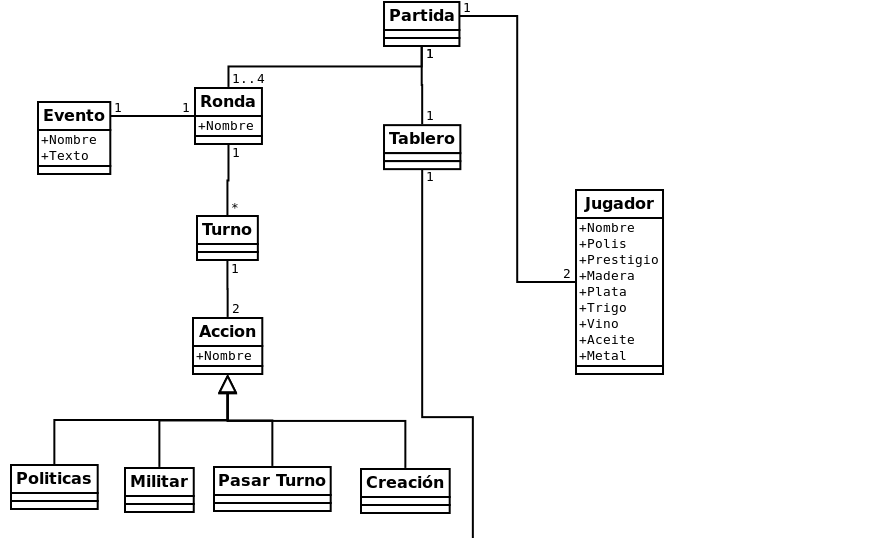
\includegraphics[width=500px]{analysis-uml/iteration2/part1.png}
			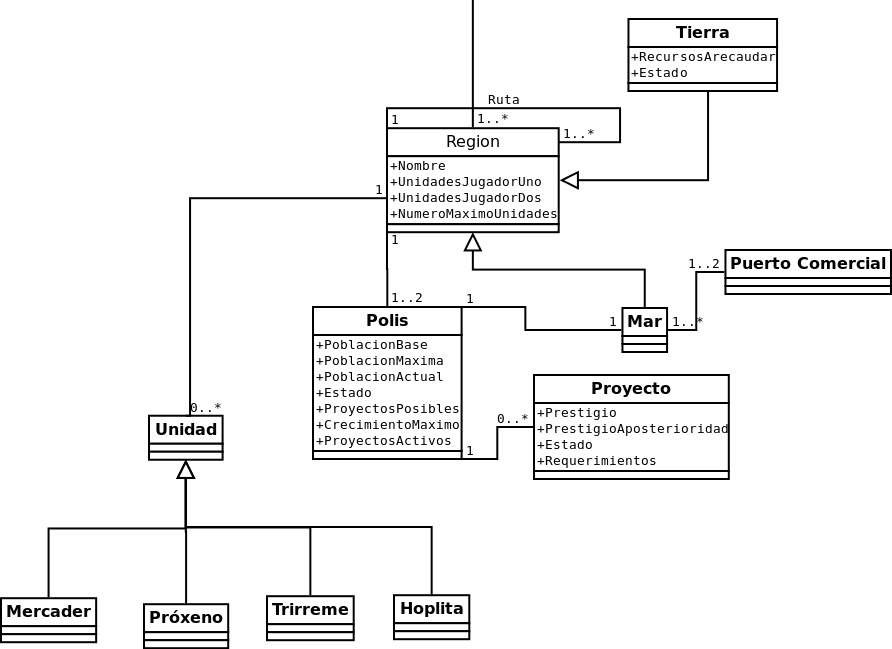
\includegraphics[width=500px]{analysis-uml/iteration2/part2.png}
		\end{center}
	\section*{Iteración 3}
		\begin{center}
			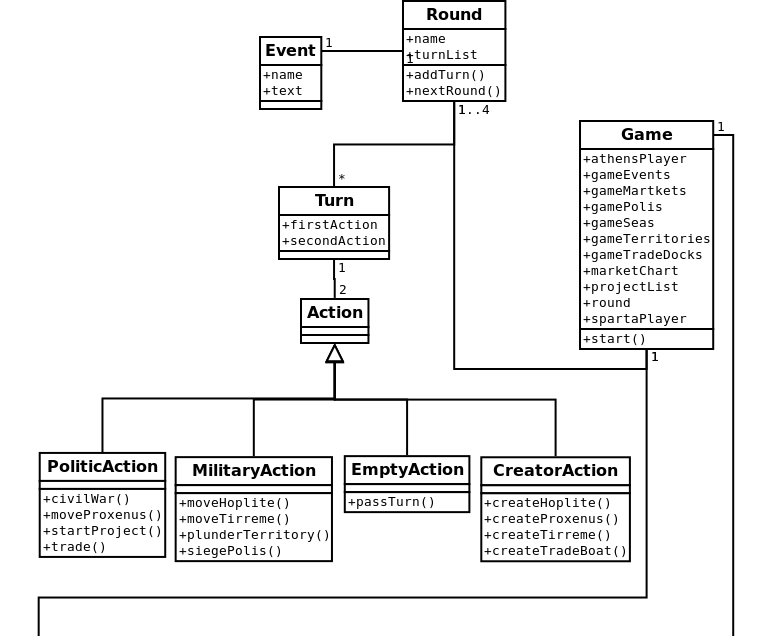
\includegraphics[width=500px]{analysis-uml/iteration3/part1.png}
			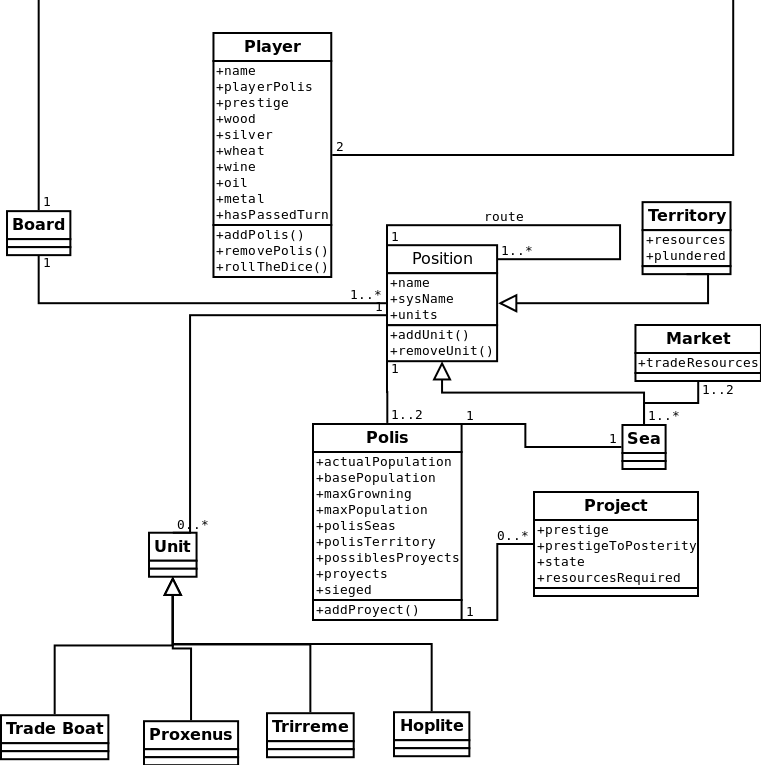
\includegraphics[width=500px]{analysis-uml/iteration3/part2.png}
		\end{center}
	
\chapter{Asignación de Responsabilidades}
		\section*{Iteración 3}
			Nota: Hemos considerado como IU cuando no sólo llama directamente a un método de interfaz para comunicarse con el usuario, sino también cuando es el método que en su interior llamará al método concreto de interfaz de usuario.

			\begin{center}
				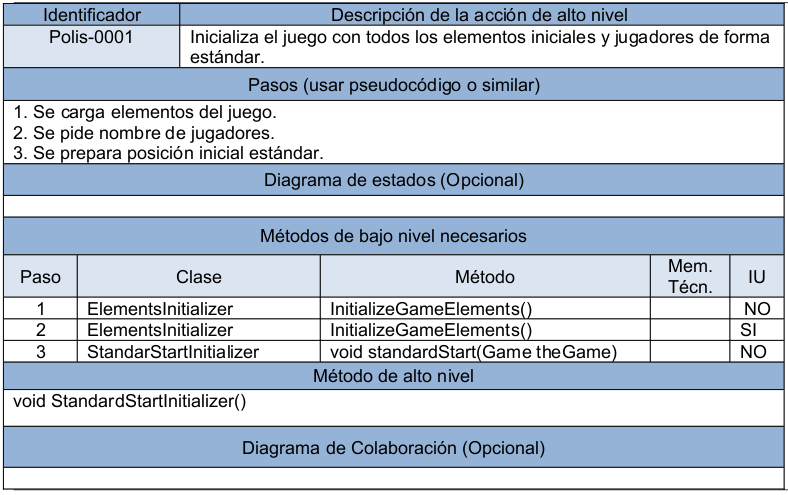
\includegraphics[width=500px]{responsabilities-allocation/iteration3/polis-0001.png}
				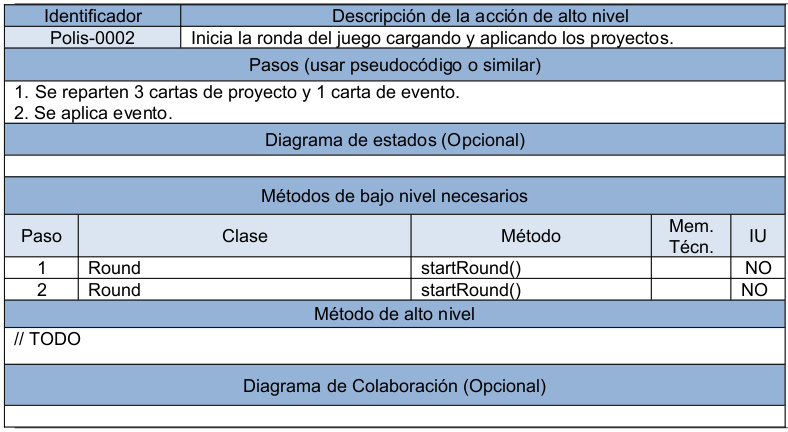
\includegraphics[width=500px]{responsabilities-allocation/iteration3/polis-0002.png}
				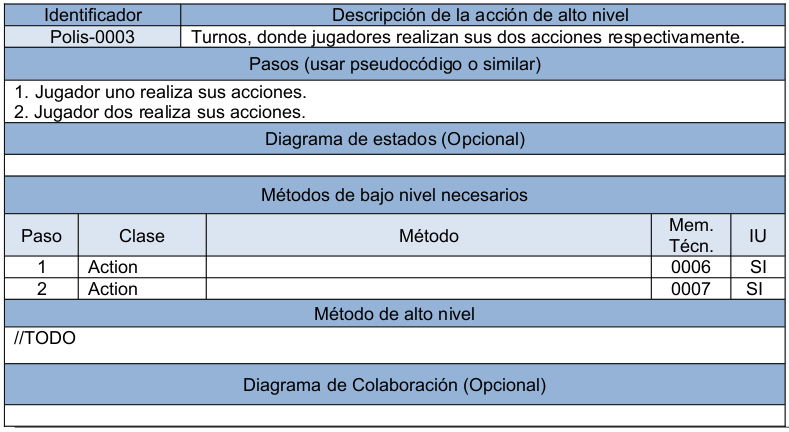
\includegraphics[width=500px]{responsabilities-allocation/iteration3/polis-0003.png}
				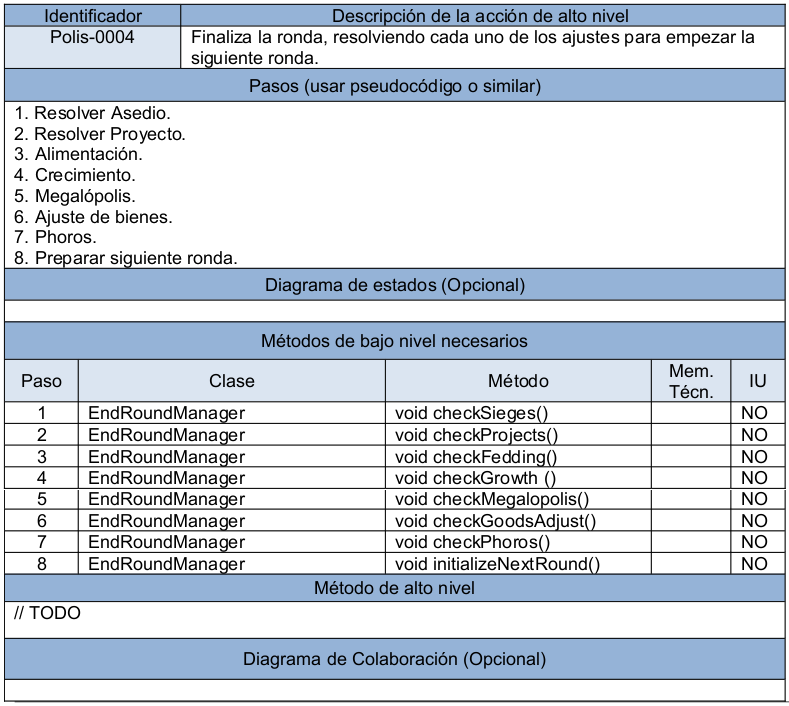
\includegraphics[width=500px]{responsabilities-allocation/iteration3/polis-0004.png}
				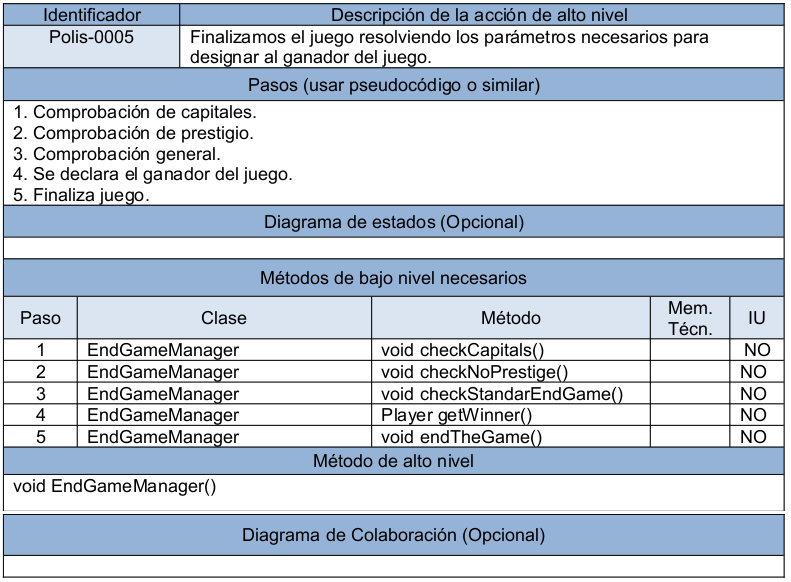
\includegraphics[width=500px]{responsabilities-allocation/iteration3/polis-0005.png}
				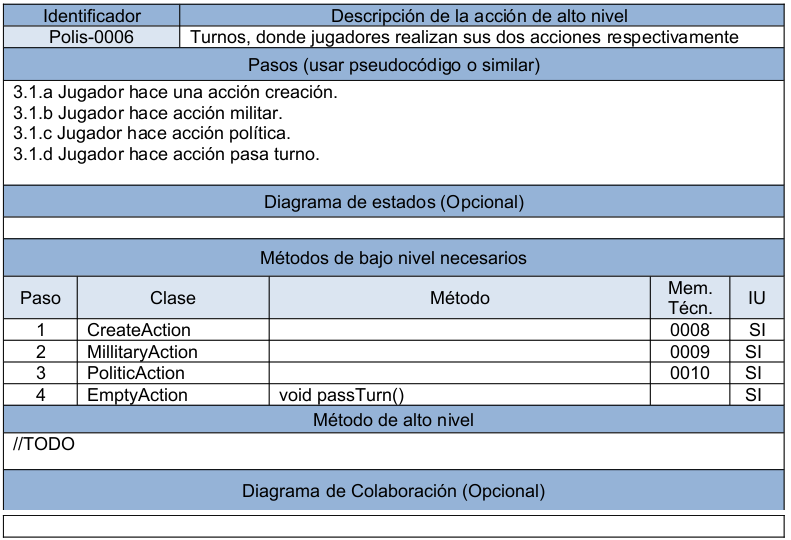
\includegraphics[width=500px]{responsabilities-allocation/iteration3/polis-0006.png}
				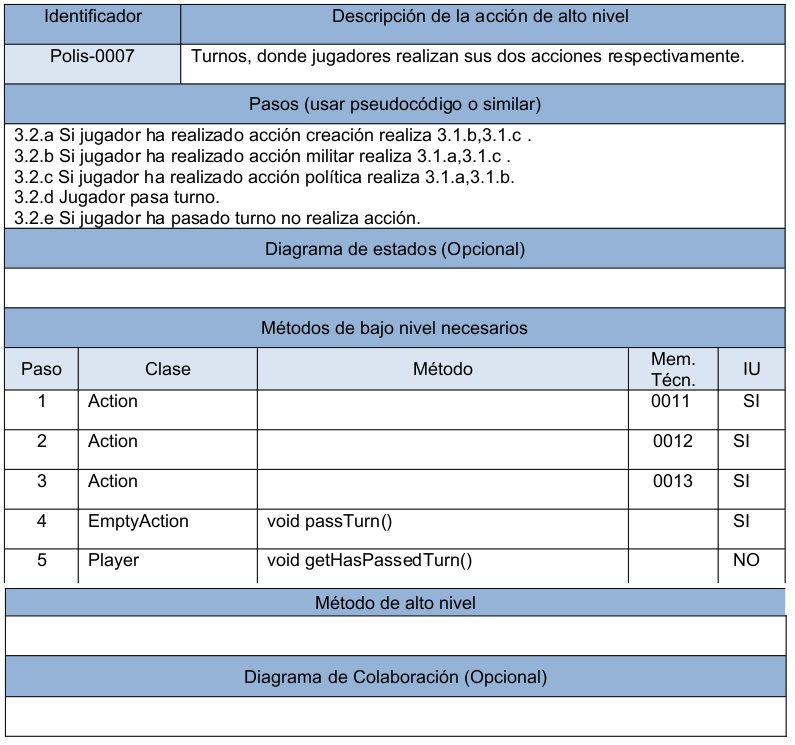
\includegraphics[width=500px]{responsabilities-allocation/iteration3/polis-0007.png}
				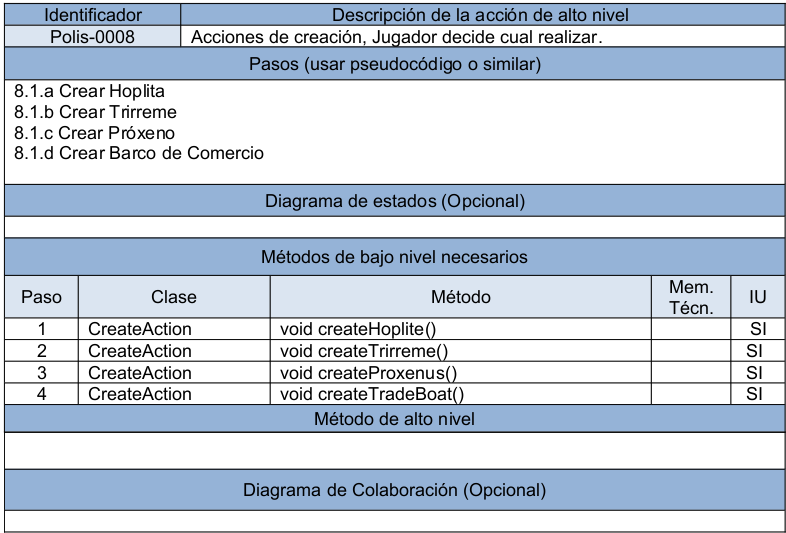
\includegraphics[width=500px]{responsabilities-allocation/iteration3/polis-0008.png}
				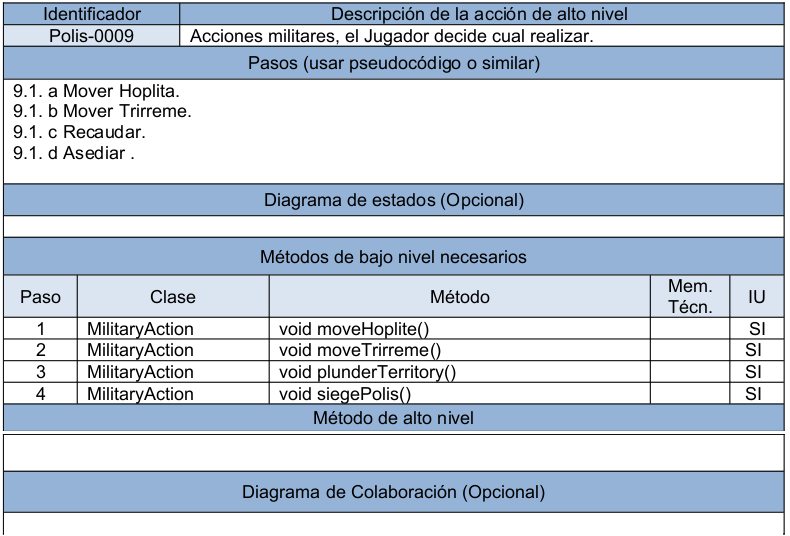
\includegraphics[width=500px]{responsabilities-allocation/iteration3/polis-0009.png}
				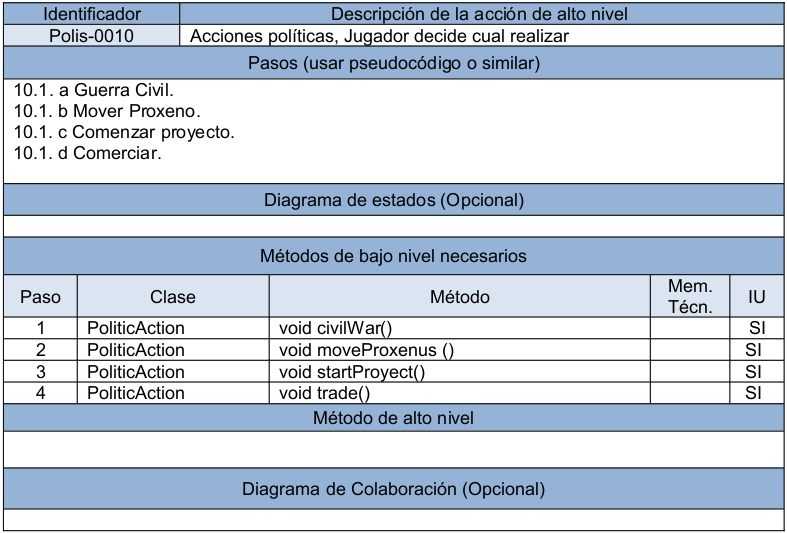
\includegraphics[width=500px]{responsabilities-allocation/iteration3/polis-0010.png}
				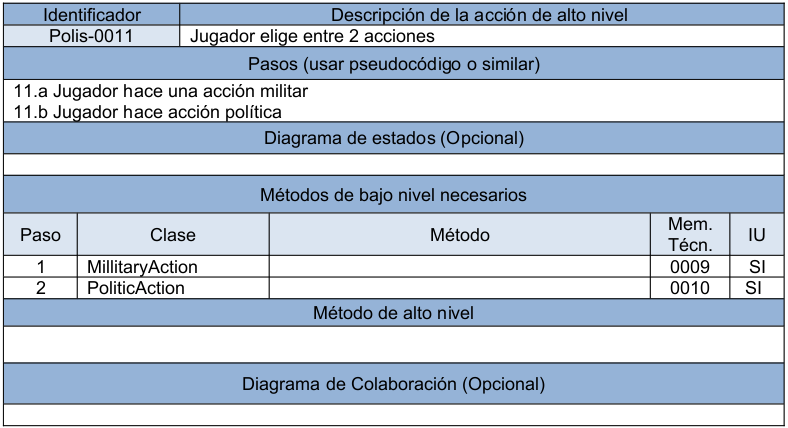
\includegraphics[width=500px]{responsabilities-allocation/iteration3/polis-0011.png}
				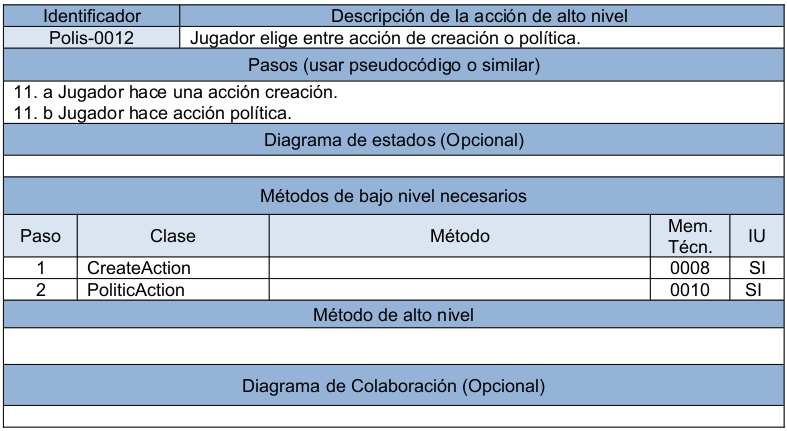
\includegraphics[width=500px]{responsabilities-allocation/iteration3/polis-0012.png}
				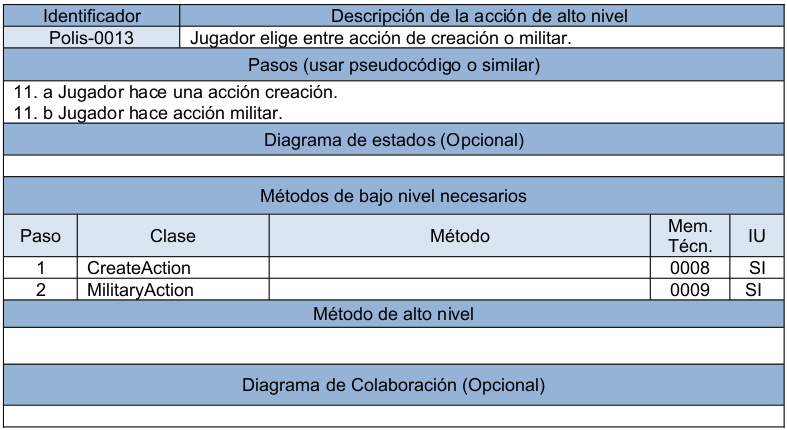
\includegraphics[width=500px]{responsabilities-allocation/iteration3/polis-0013.png}
			\end{center}
		\section*{Iteración 4}
			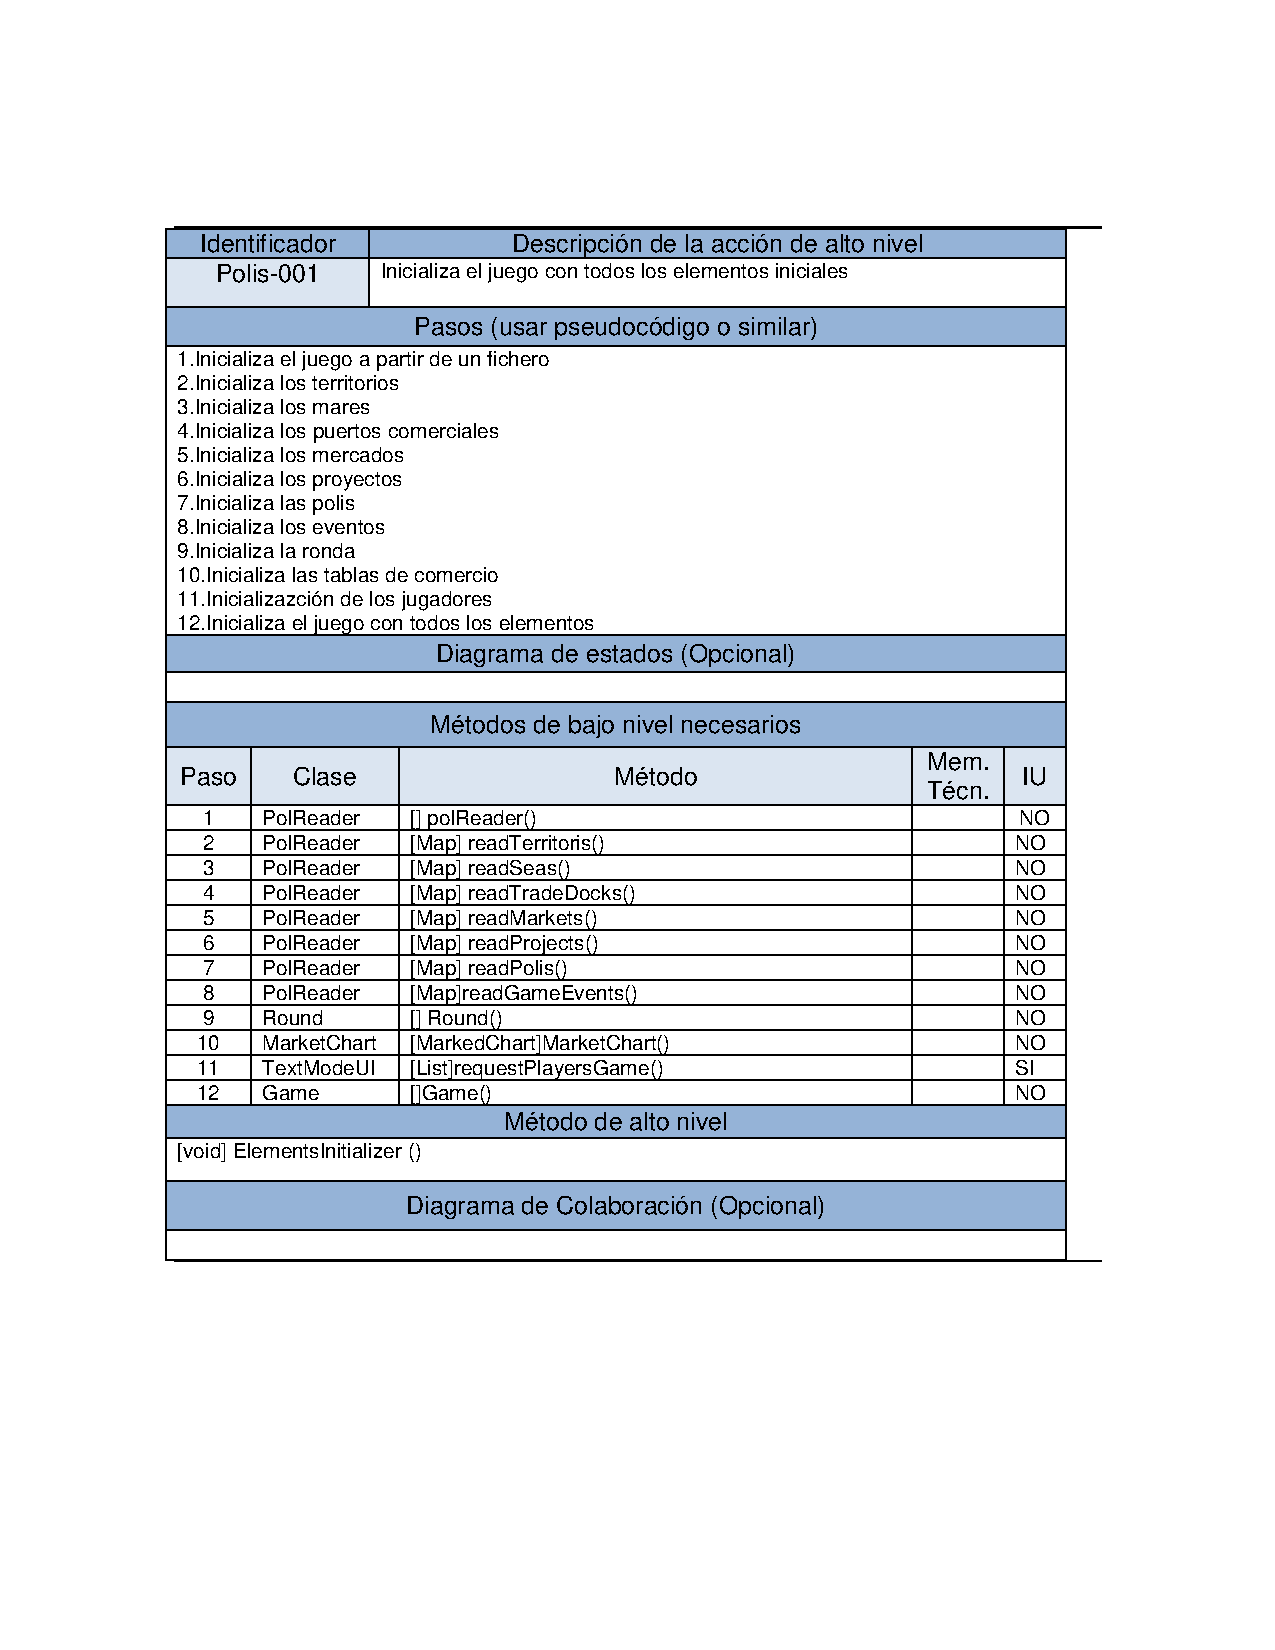
\includepdf[pages=-]{responsabilities-allocation/iteration4/dar.pdf}
\chapter{Diagrama UML de Diseño}
	\section*{Iteración 3}
		\begin{center}
		    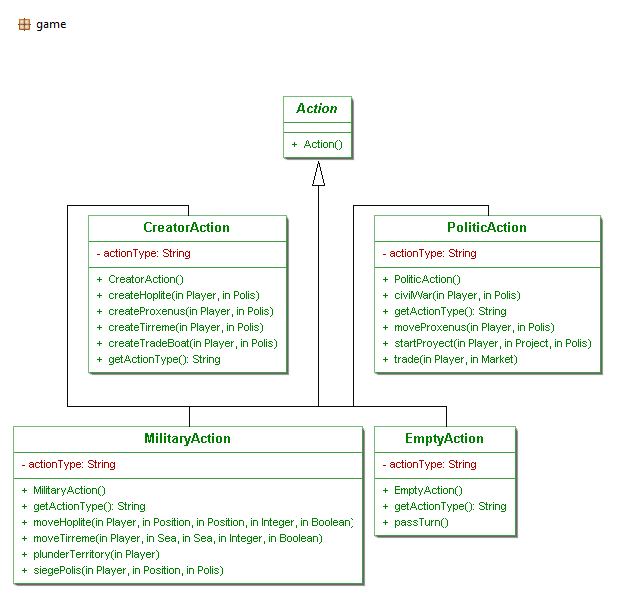
\includegraphics[width=500px]{design-uml/iteration3/game-actions.png}
		    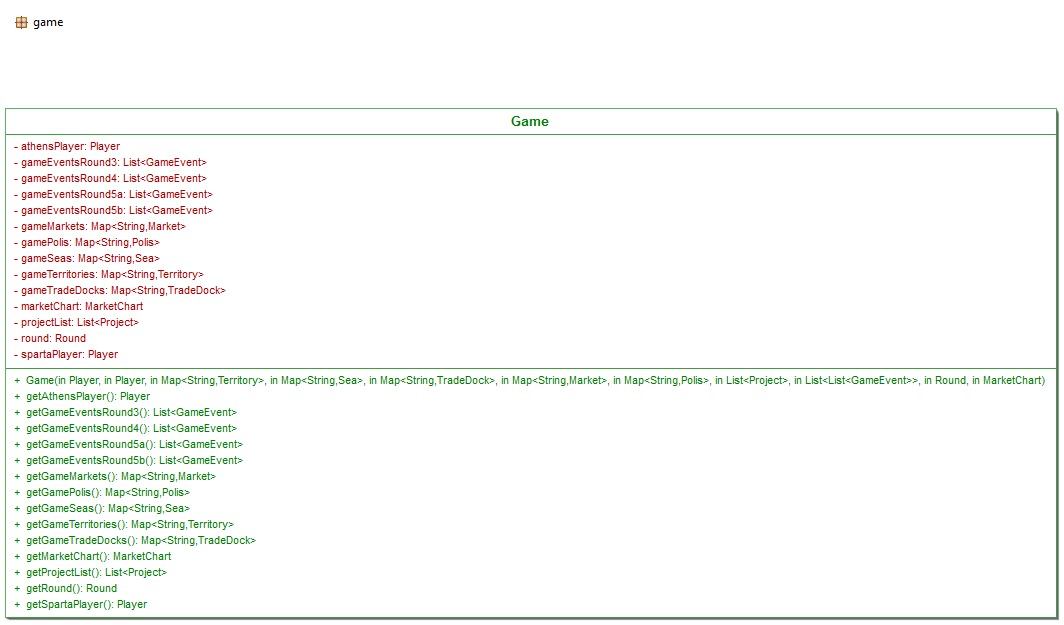
\includegraphics[width=500px]{design-uml/iteration3/game-game.png}
		    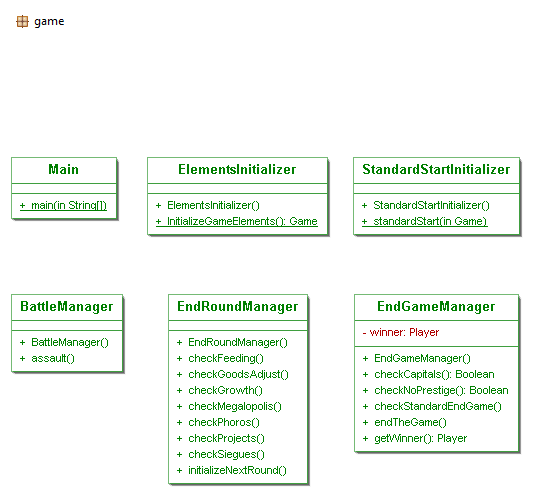
\includegraphics[width=500px]{design-uml/iteration3/game-main-managers.png}
		    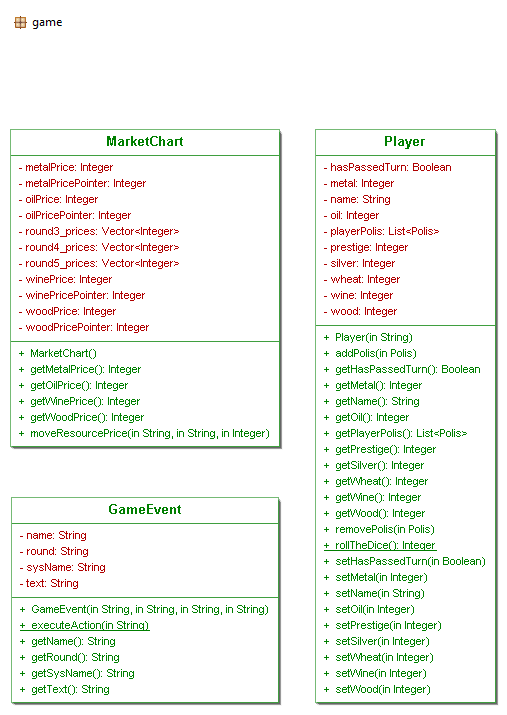
\includegraphics[width=500px]{design-uml/iteration3/game-martket-gameevent-player.png}
		    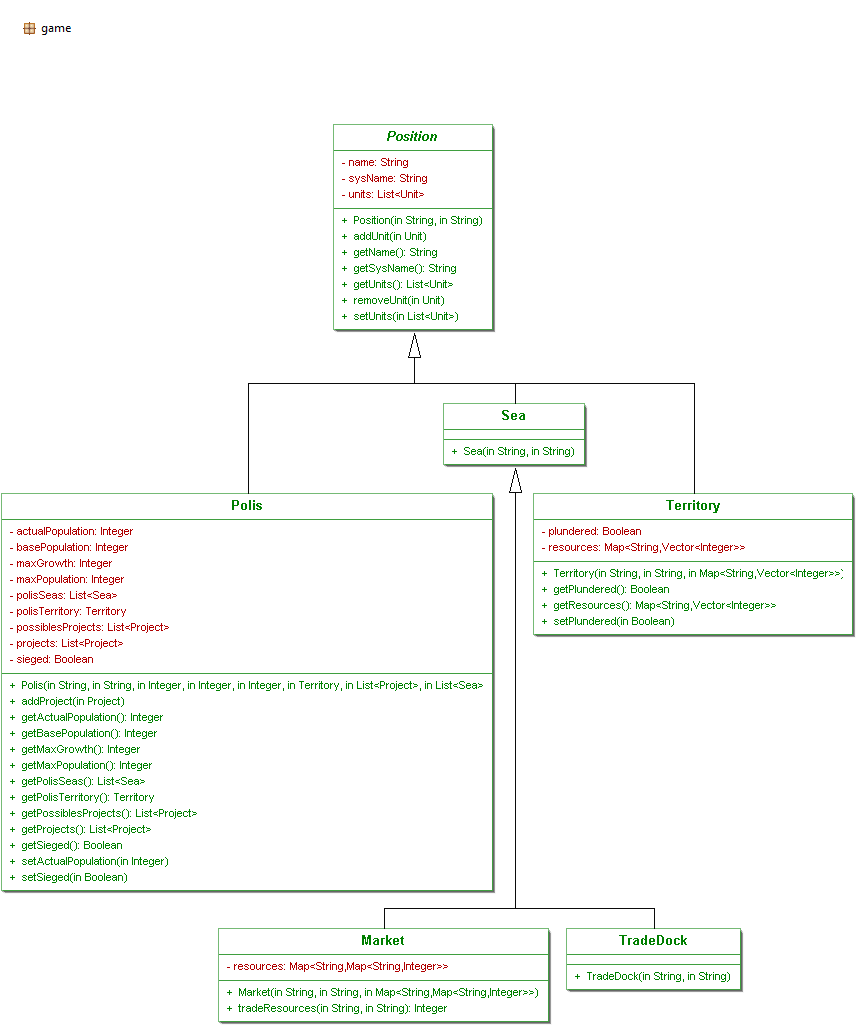
\includegraphics[width=500px]{design-uml/iteration3/game-positions.png}
		    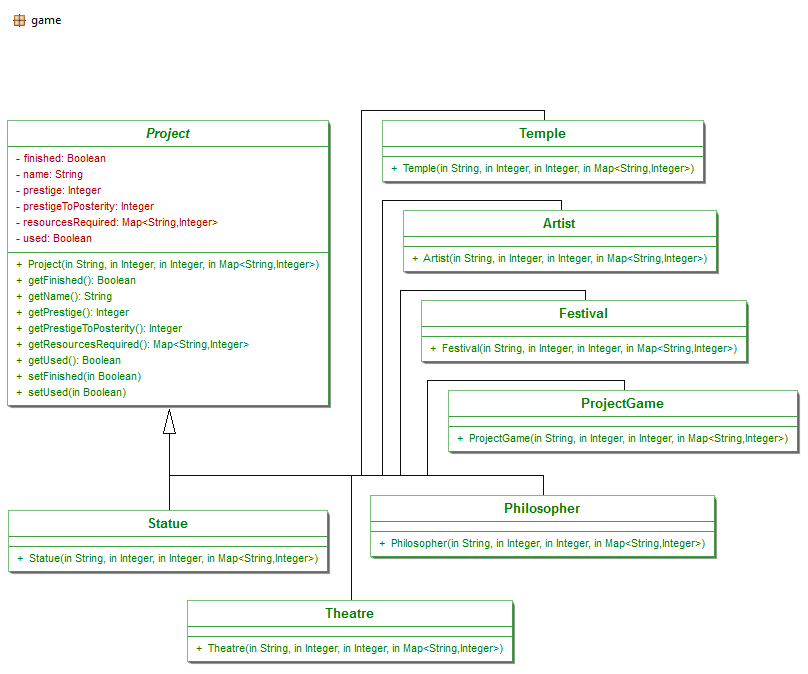
\includegraphics[width=500px]{design-uml/iteration3/game-projects.png}
		    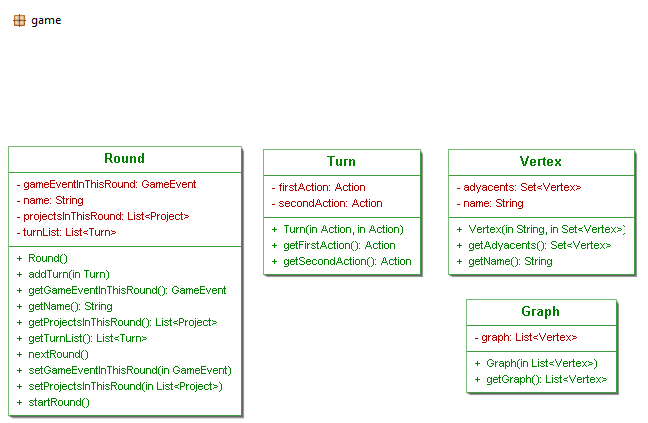
\includegraphics[width=500px]{design-uml/iteration3/game-round-turn-graph-vertex.png}
		    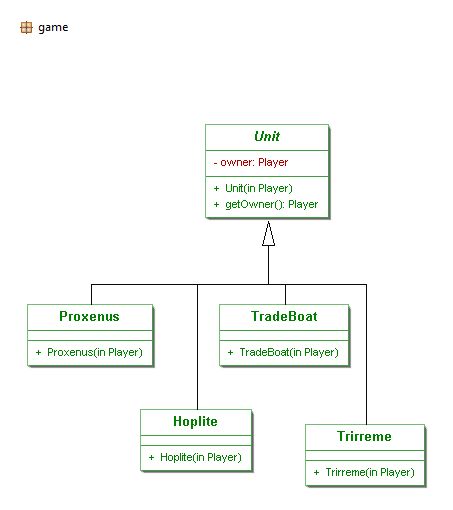
\includegraphics[width=500px]{design-uml/iteration3/game-units.png}
		    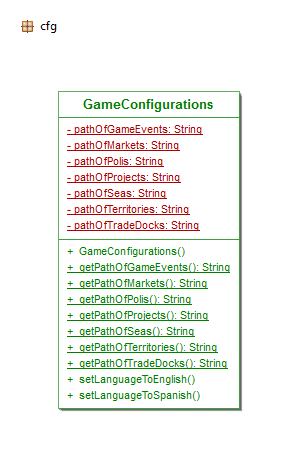
\includegraphics[width=500px]{design-uml/iteration3/package-cfg.png}
		    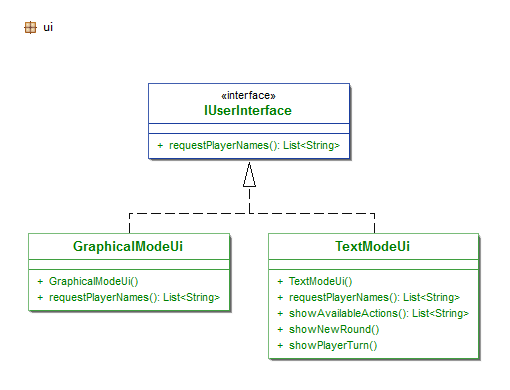
\includegraphics[width=500px]{design-uml/iteration3/package-ui.png}
		    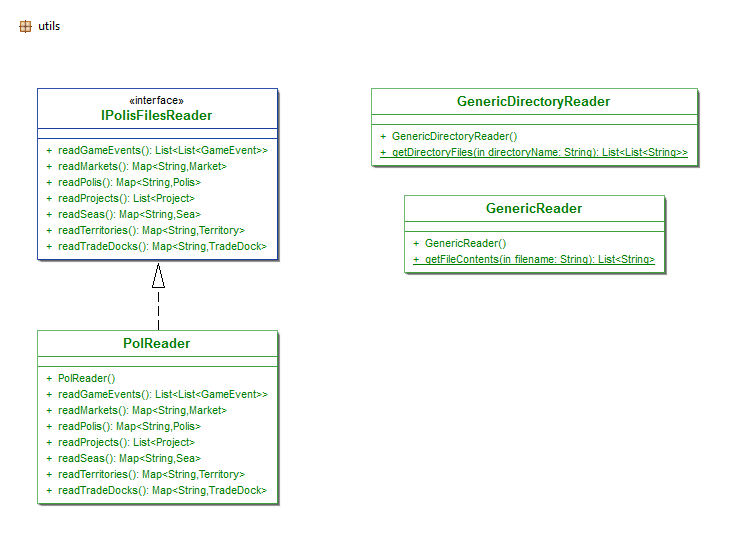
\includegraphics[width=500px]{design-uml/iteration3/package-utils.png}
		\end{center}    
\end{document}

